\documentclass[10pt]{beamer}
\usepackage{iftex}
\ifPDFTeX
\usepackage[T2A]{fontenc}
\usepackage[utf8]{inputenc} % Кодировка utf-8, cp1251 и т.д.
\usepackage[english,russian]{babel}
\else
  \RequirePackage{polyglossia}
  \RequirePackage{luatextra}
  \defaultfontfeatures{Ligatures=TeX,Numbers=Lining,Scale=MatchLowercase}

  \setmainfont{Times New Roman}
  \setsansfont{Calibri}
  \setmonofont{Fira Code}

  %\setmathfont{Cambria Math}%

  \newfontfamily{\cyrillicfont}{Times New Roman}
  \newfontfamily{\cyrillicfontrm}{Times New Roman}
  \newfontfamily{\cyrillicfonttt}{Fira Code}
  \newfontfamily{\cyrillicfontsf}{Fira Sans Regular}
\fi

\usepackage{amsmath,amssymb,longtable,hhline}
\usepackage{mathrsfs}
\usepackage{xcolor}
\usepackage{listings}
\usepackage{hyperref}
\usepackage{multicol}
\usepackage{anyfontsize}
\usepackage{minted}
%\usepackage{enumitem}

% \setlist[description]{leftmargin=0pt,labelindent=\parindent}

\usemintedstyle{tango}
\newcommand{\ltprgsize}{\fontsize{5}{5}\selectfont}
\newcommand{\btprgsize}{\fontsize{7}{7}\selectfont}
\setminted{fontsize=\ltprgsize,mathescape}

\definecolor{mygreen}{rgb}{0,0.6,0}
\definecolor{mygray}{rgb}{0.5,0.5,0.5}
\definecolor{mymauve}{rgb}{0.58,0,0.82}

\hypersetup{
    bookmarks=true,         % show bookmarks bar?
    unicode=true,           % non-Latin characters in Acrobat’s bookmarks
    pdftoolbar=false,        % show Acrobat’s toolbar?
    pdfmenubar=false,        % show Acrobat’s menu?
    pdffitwindow=false,     % window fit to page when opened
    pdfstartview={FitH},    % fits the width of the page to the window
    pdftitle={Компьютерная алгебра в задачах оптимизации},    % title
    pdfauthor={Evgeny Cherkashin, Seseg Badmatsyrenova},     % author
    pdfsubject={symbolic computations},   % subject of the document
    pdfnewwindow=true,      % links in new PDF window
    colorlinks=true,       % false: boxed links; true: colored links
    linkcolor=red,          % color of internal links (change box color with linkbordercolor)
    citecolor=green,        % color of links to bibliography
    filecolor=magenta,      % color of file links
    urlcolor=blue           % color of external links
}

\lstset{language=Python,
  basicstyle=\footnotesize\ttfamily,        % the size of the fonts that are used for the code
  breakatwhitespace=false,         % sets if automatic breaks should only happen at whitespace
  breaklines=true,                 % sets automatic line breaking
  captionpos=b,                    % sets the caption-position to bottom
  commentstyle=\color{mygreen},    % comment style
  escapeinside={\%*}{*)},          % if you want to add LaTeX within your code
  extendedchars=true,              % lets you use non-ASCII characters; for 8-bits encodings only, does not work with UTF-8
%  frame=single,                    % adds a frame around the code
  keepspaces=true,                 % keeps spaces in text, useful for keeping indentation of code (possibly needs columns=flexible)
  keywordstyle=\color{blue},       % keyword style
%  numbers=left,                    % where to put the line-numbers; possible values are (none, left, right)
  numbersep=5pt,                   % how far the line-numbers are from the code
  numberstyle=\tiny\color{mygray}, % the style that is used for the line-numbers
  rulecolor=\color{black},         % if not set, the frame-color may be changed on line-breaks within not-black text (e.g. comments (green here))
  showspaces=false,                % show spaces everywhere adding particular underscores; it overrides 'showstringspaces'
  showstringspaces=false,          % underline spaces within strings only
  showtabs=false,                  % show tabs within strings adding particular underscores
  stepnumber=2,                    % the step between two line-numbers. If it's 1, each line will be numbered
  stringstyle=\color{mymauve},     % string literal style
  tabsize=2,                       % sets default tabsize to 2 spaces
%  title=\lstname                   % show the filename of files included with \lstinputlisting; also try caption instead of
}
\usepackage{pifont}

\usetheme{Warsaw}
\usecolortheme{crane}
%\useinnertheme{rectangles}
\setbeamertemplate{itemize item}{\scriptsize\hbox{\donotcoloroutermaths\ding{113}}}
\setbeamertemplate{itemize subitem}{\tiny\raise1.5pt\hbox{\donotcoloroutermaths$\blacktriangleright$}}
\setbeamertemplate{itemize subsubitem}{\tiny\raise1.5pt\hbox{\donotcoloroutermaths$\blacktriangleright$}}
\setbeamertemplate{enumerate item}{\insertenumlabel.}
\setbeamertemplate{enumerate subitem}{\insertenumlabel.\insertsubenumlabel}
\setbeamertemplate{enumerate subsubitem}{\insertenumlabel.\insertsubenumlabel.\insertsubsubenumlabel}
\setbeamertemplate{enumerate mini template}{\insertenumlabel}

\beamertemplatenavigationsymbolsempty

\usepackage{iftex,ifxetex}
\ifPDFTeX
  \usepackage[utf8]{inputenc}
  \usepackage[T1]{fontenc}
  \usepackage[russian]{babel}
  \usepackage{lmodern}
  \usefonttheme{serif}
\else
  \ifluatex
    \usepackage{unicode-math}
    \defaultfontfeatures{Ligatures=TeX,Numbers=OldStyle}
    \setmathfont{Latin Modern Math}
    \setsansfont{Linux Biolinum O}
    \setmonofont{Fira Code}
    \usefonttheme{professionalfonts}
    % \setmathfont[
    %     Ligatures=TeX,
    %     Scale=MatchLowercase,
    %     math-style=upright,
    %     vargreek-shape=unicode
    %     ]{euler.otf}
  \fi
\fi

%\useoutertheme{split}
%\useinnertheme{rounded}
\setbeamertemplate{background canvas}[vertical shading][bottom=white!80!cyan!20,top=cyan!10]
%\setbeamertemplate{sidebar canvas left}[horizontal shading][left=white!40!black,right=black]

\graphicspath{{pics/}}


% --------------------------
\newcommand{\GB}[1]{\colorbox{green}{#1}}
\newcommand{\BB}[1]{\colorbox{blue}{#1}}
\newcommand{\RB}[1]{\colorbox{red}{#1}}
\usepackage{changepage}

\begin{document}
\title{Digital Archives Supporting Document Content Inference}
%\title[Digital archives with AI]{Digital Archives Supporting Document Content Inference}
\author[E.~Cherkashin, A.~Shigarov, V.~Paramonov, A.~Mikhailov]{Evgeny Cherkashin,
Alexey Shigarov,\\
Viacheslav Paramonov,
Andrey Mikhailov}
\institute[ISDCT SB RAS]{V.M. Matrosov's Institute of System Dynamics and Control Theory SB RAS}
\date[2019]{{}\\[1.5cm]
CIS, MIPRO-42,
20-24 May 2019, Opatija, Croatia
}
%\date{\today}
\maketitle

\begin{frame}
  \frametitle{Document authoring and storage}
  In most cases documents are created as a result of
  \begin{itemize}
  \item creative activity of a person with a text processors (authoring);
  \item printing a digital copy or a data record in a database;
  \item aggregation operation over database records (report).
  \end{itemize}
  Then it is stored either as a physical paper and/or a digital document (PDF, DOCX, HTML).

  Since 2000-th, Semantic Web and Linked Open Data (LOD) is being developed, allowing
  \begin{itemize}
  \item structural storage of data within published documents;
  \item processing stored data computationally;
  \item integration of data structures and data objects globally.
  \end{itemize}

  The \textbf{aim of this research} is to develop technologies, software and services allowing construction of digital archives supporting document data inclusion and inference from existing documents.
\end{frame}

\begin{frame}
  \frametitle{Structure of a document}
  \centering
  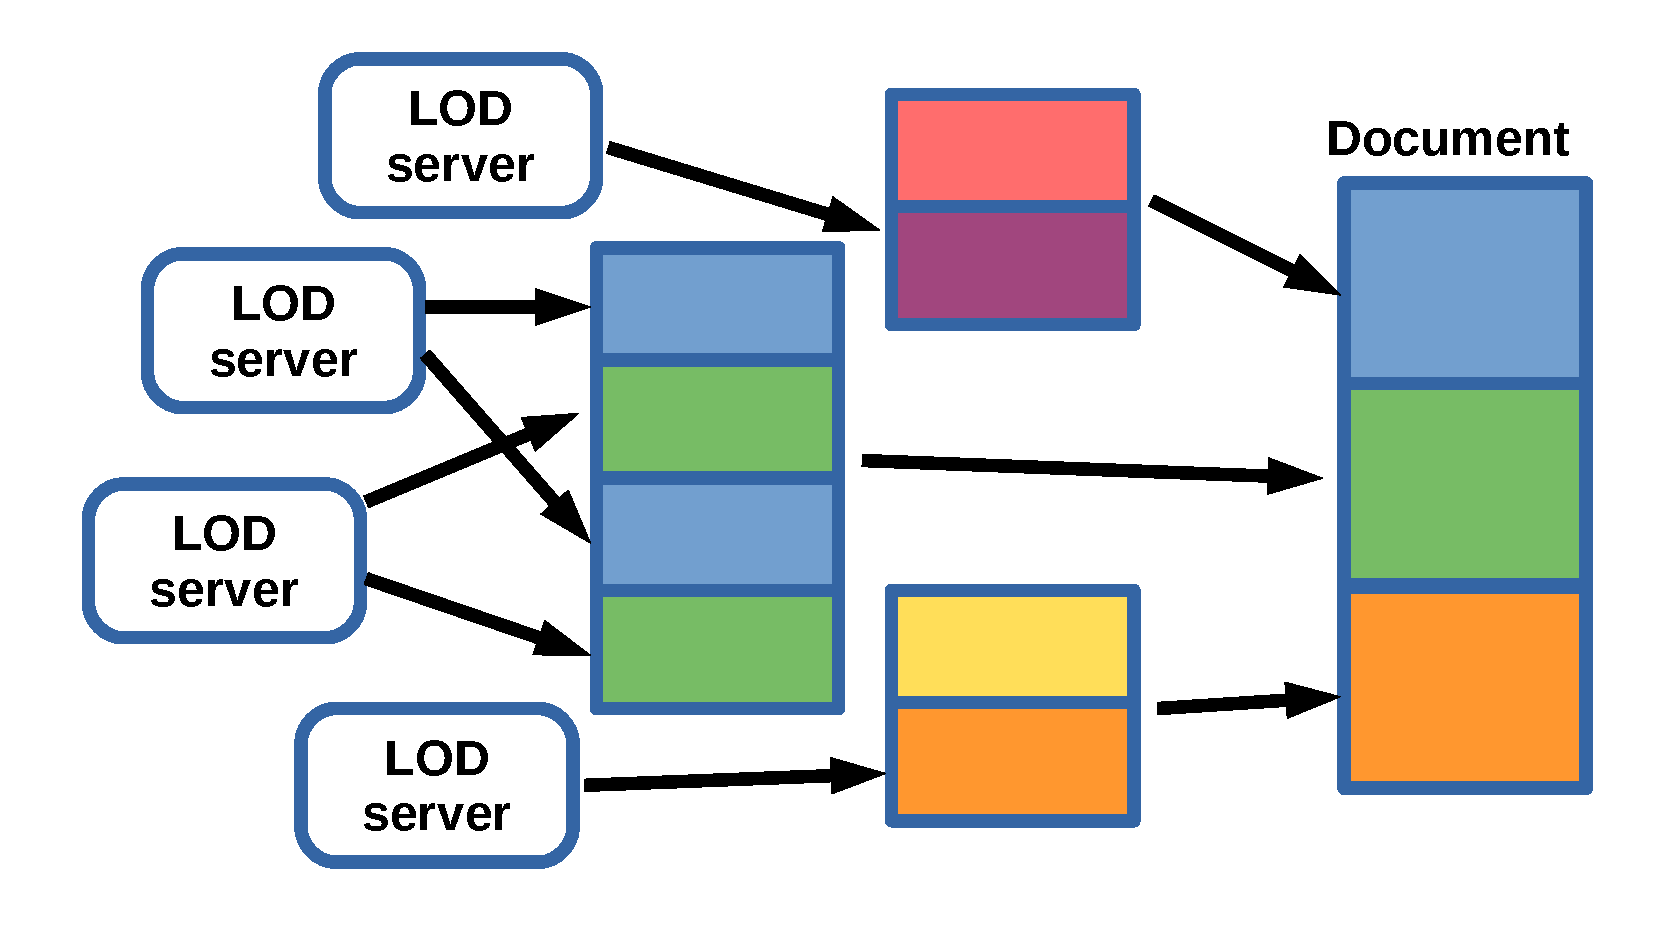
\includegraphics[width=1\linewidth]{document-structural-view.pdf}
\end{frame}

\begin{frame}
  \frametitle{Linked Open Data, LOD}
  \begin{enumerate}
  \item Information is published in Internet with open access license;
  \item It is represented in a machine-readable form, e.g., Excel table instead of a bitmap picture;
  \item An open format used, e.g., CSV instead of Excel;
  \item The format is based on W3C recommended standards, allowing RDF and SPARQL reference;
  \item Published data refer to objects, forming context.
  \end{enumerate}
  Thus, applications publish data as relations of objects (entities)
\end{frame}

\begin{frame}
  \frametitle{Open Annotaiton (oa)}
\begin{adjustwidth}{-3em}{-3em}
  \centering
  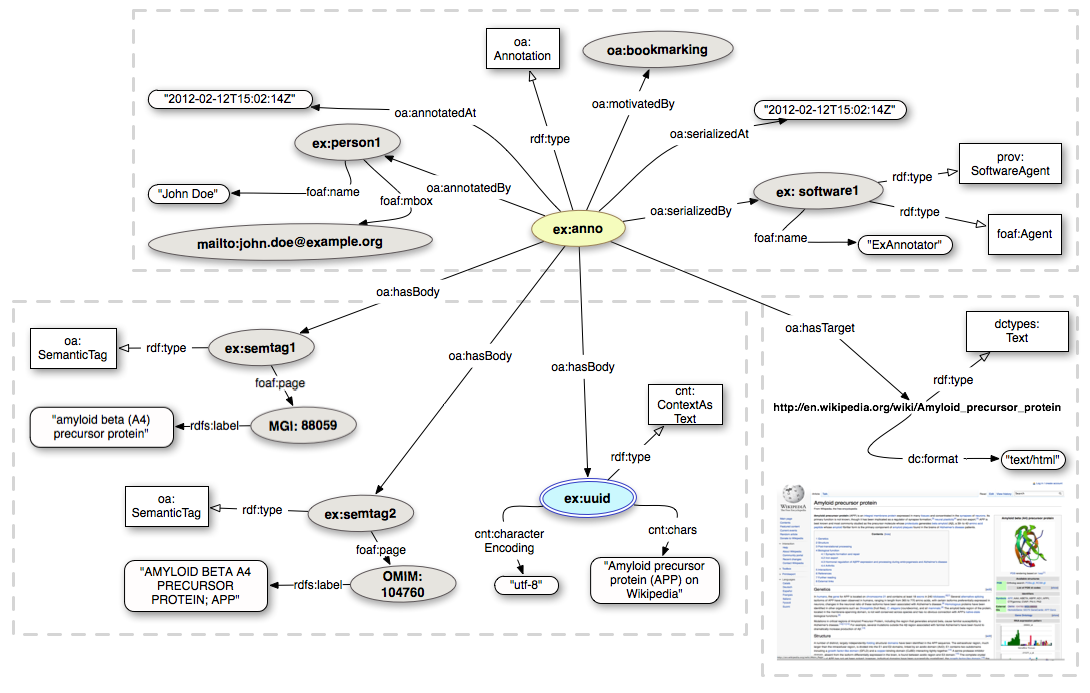
\includegraphics[width=1\linewidth]{Open-Annotation_CB_Bookmarking_and_Semantically_Tagging_A_webpage_spec20130128.png}
\end{adjustwidth}

\end{frame}

\begin{frame}[fragile,fragile]
  \frametitle{Representation}
  % \begin{block}{}
  %   \textbf{Целью} исследования является создание методики разработки процедур трансформации (PD\footnote{Platform [description] model.}) в виде ОО-модулей.
  % \end{block}
  % \begin{columns}
  %   \begin{column}{0.5\linewidth}
  %     % \includegraphics[width=1\linewidth]{pics/scenario-ru-wo-mothur.pdf}
  %   \end{column}
  %   \begin{column}{0.6\linewidth}
  %     Задачи исследования:
  %     \begin{itemize}
  %     \item Изучить синтаксические структуры Logtalk в аспекте структурирования знаний;
  %     \item Предложить методику представления трансформации в виде ОО-модулей;
  %     \item Реализовать библиотеку объектов и классов для МДА;
  %     \item Тестирование библиотеки на примере.
  %     \end{itemize}
  %   \end{column}
  % \end{columns}

\begin{adjustwidth}{-1.5em}{-1.5em}
\begin{minted}[escapeinside=||,fontsize=\btprgsize]{xml}
<html lang="ru" xmlns=http://www.w3.org/1999/xhtml
|\GB{xmlns:taa}|=http://irnok.net/engine/rdfa-manipulation
xml:lang="ru" metal:define-macro="page">
<head> . . . . </head>
<body prefix="rdf: http://www.w3.org/1999/...-ns# foaf: http://xmlns.com/foaf/...
imei: imei.html# course: https://irnok.net/college/plan/01..16-...\
%D0\%BA_PB-SM.plm.xml.xlsx-....2.3.1.html#"  resource="#post"
typeof="schema:CreativeWork sioc:Post prov:Entity">
<!-- The application control panel -->

<main lang="ru" resource="#annotation" typeof="oa:Annotation" id="main-doc-cnt">
<div property="oa:hasTarget" resource="#course-work-prog"></div>
<article property="oa:hasBody" typeof="foaf:Document curr:WorkingProgram"
         resource="#course-work-program" id="main-document">
  <div |\GB{taa:content}|="imei:title-page"></div>
  <div |\GB{taa:content}|="imei:neg-UMK"></div>
  <section id="TOC" class="break-after"> <h2>Table of Contents</h2>
    <div id="tableOfContents"></div>
  </section>
  <section id="course-description" resource="#description"
           property="schema:hasPart" typeof="schema:CreativeWork">
    <div property="schema:hasPart" resource="#purpose"
         typeof="dc:Text cnt:ContentAsText" >
      <div property="cnt:chars" datatype="xsd:string">
        <h2 property="dc:title" datatype="xsd:string">
           Aims and objectives of the discipline (module)</h2>
        <p>The aim of teaching the discipline ...</p>
      </div>
   </div>
  . . . . . . . .
\end{minted}
\end{adjustwidth}
\end{frame}

\begin{frame}
  \frametitle{Architecture}
  \begin{adjustwidth}{-2.5em}{-2.5em}
    \begin{center}
      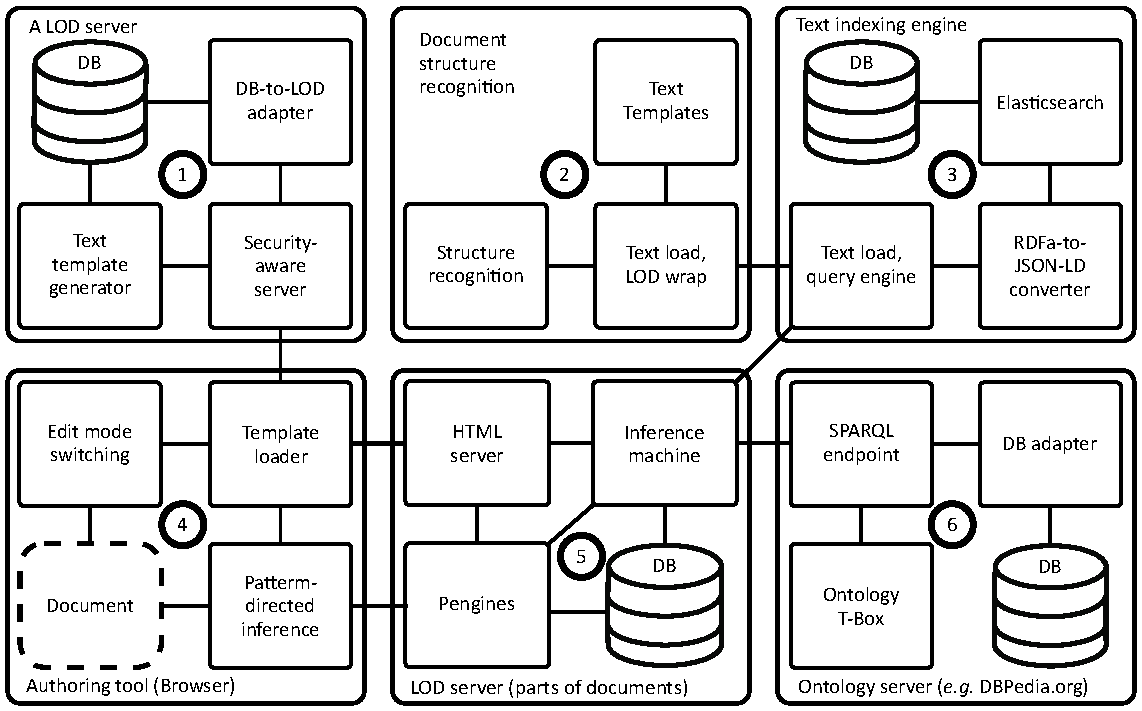
\includegraphics[width=1\linewidth]{architecture-mda-lod-ext.pdf}
    \end{center}
  \end{adjustwidth}

% \begin{itemize}
% \item content and metadata repository with SPARQL (6) and full-text search (3); the engines for LOD processing (5) based on the logical inference;
% \item service for analysis of the stored content (2) enriching the archive with semantic information describing the content;
% \item tools for development of LOD applications and their user interfaces (1);
% \item browser based authoring tools (4).
% \end{itemize}
\end{frame}

\begin{frame}
  \frametitle{Generated list of title page preambles}
    \begin{adjustwidth}{-2.5em}{-2.5em}
    \begin{center}
      
\includegraphics[width=0.7\linewidth]{template-title-pages.jpg}
    \end{center}
  \end{adjustwidth}
\end{frame}

\begin{frame}
  \frametitle{Generated part of study program}
   \begin{adjustwidth}{-2.5em}{-2.5em}
    \begin{center}
      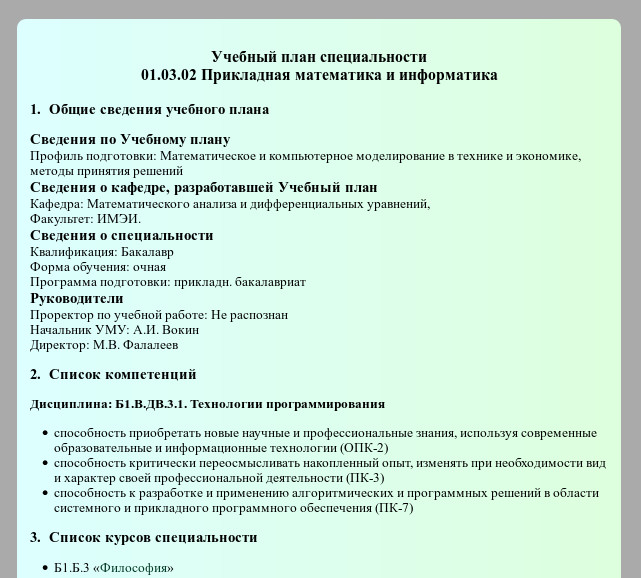
\includegraphics[width=0.7\linewidth]{template-courses.jpg}
    \end{center}
  \end{adjustwidth}
\end{frame}
\begin{frame}
  \frametitle{Imported distribution of lecture, seminary, lab hours}
   \begin{adjustwidth}{-2.5em}{-2.5em}
    \begin{center}
      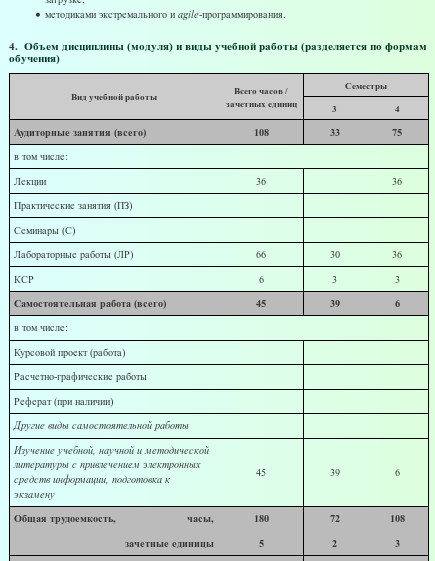
\includegraphics[width=0.9\linewidth]{work-program-volume.jpg}
    \end{center}
  \end{adjustwidth}
\end{frame}

\begin{frame}
  \frametitle{Complete document}
  \begin{adjustwidth}{-2.5em}{-2.5em}
    \begin{center}
      \begin{columns}
        \begin{column}{0.5\linewidth}
          
\includegraphics[width=1\linewidth]{work-program-title.jpg}
        \end{column}
        \begin{column}{0.5\linewidth}
          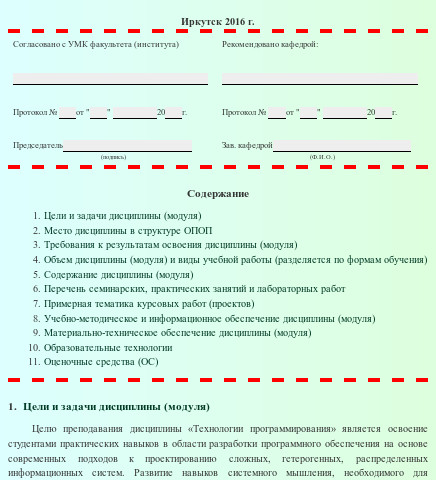
\includegraphics[width=1\linewidth]{work-program-agreement.jpg}
        \end{column}
    \end{columns}
    \end{center}
  \end{adjustwidth}
\end{frame}

\begin{frame}
  \frametitle{Used ontologies}
  \begin{itemize}
  \item Friend-of-a-friend (\textbf{foaf}) - agent information: individuals, legal entities, program agents.
  \item Provenance (\textbf{prov}) - references between documents.
  \item Dublin Core (\textbf{dc}) - edited annotation mark up.
  \item DBPedia resource (\textbf{dbr}) – references to instant objects and classes.
  \item Schema.org (\textbf{schema}) - Google, Yandex, Yahoo, \emph{etc}. searchable objects, structural elements.
  \item The Bibliographic Ontology (\textbf{bibo}) - literature reference mark up.
\end{itemize}
\end{frame}

\begin{frame}
  \frametitle{Conclusion}
A tools (components) for digital archive implementation, which allows
to device information systems and document processing services
with the following features:
\begin{itemize}
\item load LOD marked up document, extract, store in a graph and index RDF data;
\item retrieve RDF data as triples or as a result of full-text search query;
\item combine existing LOD data and its content in new documents dynamically with browser based context inference machine;
\item use server-site inference machine (Prolog) to process RDF data upon
  request from browser's part of the system;
  % \item organizes a platform for document semantic markup,
\item convert created RDFa marked up HTML5 documents into Excel and Word formats.
\end{itemize}

  \textbf{Applications}
  \begin{itemize}
  \item Document authoring automation;
  \item Context-depended editing;
  % \item Export into office formats;
  \item Self-organizing global document flows;
  \item Documents as data sources for information systems.
  \end{itemize}

\end{frame}

\begin{frame}
  \vfill
  \begin{center}
    {\Huge Thanks for Your attention!}
  \end{center}
  \vfill
  \begin{center}
    
\includegraphics[width=0.3\linewidth]{qr-frame.png}
  \end{center}
  % Исходный код (без документации) доступен на github.com: \url{https://github.com/isu-enterprise/icc.xmitransform}, \url{https://github.com/eugeneai/icc.mothurpim}.
  \url{https://github.com/eugeneai/papers-2019/raw/master/MIPRO/talk.pdf}
\end{frame}

\end{document}

%%% Local Variables:
%%% mode: latex
%%% TeX-master: t
%%% End:
